\section*{Question 3}
(1) For values of $h$ uniformly spaced over the interval [0.01, 1], the 10-fold cross-validation error $\varepsilon_{cv}$($h$) is calculated for the kernel classification estimator and is shown below in Figure 4. The cross-validation error is found to be independent of the kernel bandwidth. The misclassification error of the classifier evaluated on both the training set and the testing set is 0 in both cases. However, these conclusions could be incorrect, due to possible programming errors that result in incorrect calculations of the kernel classification estimator.
\begin{figure}[h!]
    \centering
    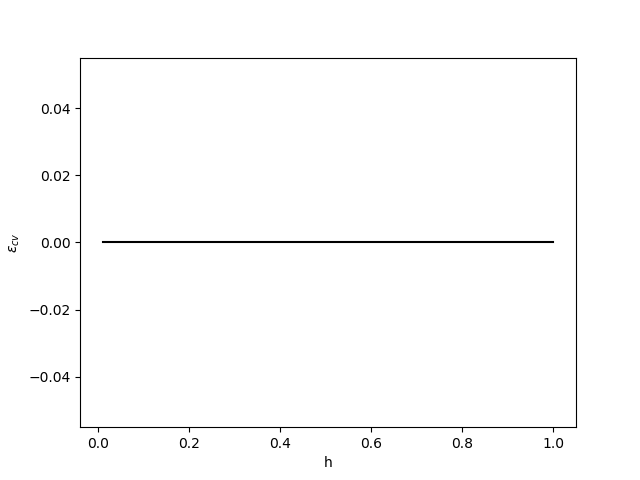
\includegraphics[height=4in]{Figure_10.png}
    \caption{Modified cross-validation error as a function of $h$ for the kernel classification estimator}
\end{figure}
\newpage
(2) If we modify the cross-validation portion of the previous question and repeat the same procedure for finding an optimal value of $h$, the optimal value can be found at (0.9802, 10.6695), as shown below in Figure 5. As the kernel bandwidth increases, the error decreases and converges to minimum value. Similar to the previous question, the misclassification error of the classifier evaluated on both the training set and the testing set is 0 in both cases. Again, this could be due to possible programming errors.

\begin{figure}[h!]
    \centering
    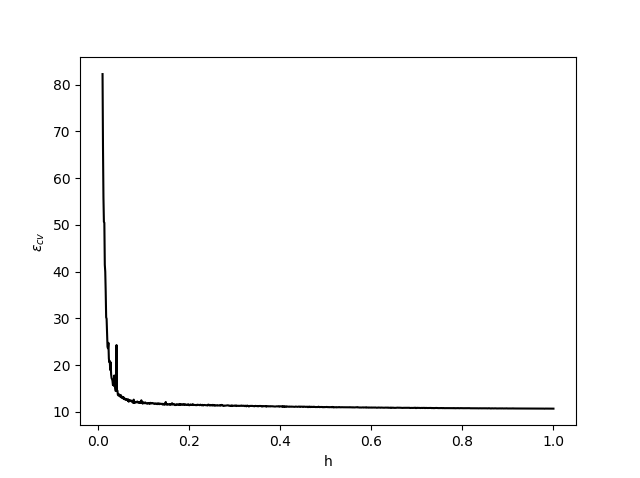
\includegraphics[height=4in]{Figure_11.png}
    \caption{Cross-validation error as a function of $h$ for the kernel classification estimator}
\end{figure}

*Note: The files submitted for this assignment also include the 3 programs that were used to generate figures and important values. The programs were written using Python 2.7 and use modules that are included in Anaconda.